\subsection{Introduction}

In this crucial section of my thesis, I explore the pragmatic aspects of the implementation process, revealing the manner in which my proposed solution was actualized. The proposed solution incorporates a comprehensive system consisting of four essential components: a MongoDB database, an ASP.NET API, an Angular web application designed for administrative purposes, and a .NET MAUI mobile application that is compatible with both iPhone and Android devices. The purpose of this section is to offer a comprehensive explanation of each module, elucidating their respective contributions to the overall software solution.

The sections on each part of my solution will start with a reason why I chose each technology. Included are discussions on why MongoDB was chosen as the database, the benefits of using ASP.NET to create the API, the choice of Angular for the web app, and the advantages of using.NET MAUI to create cross-platform mobile apps. The evaluation is not only about the choice, but also about how these technologies work together to make a system that works as a whole.

I will also carefully look over all the details of the implementation process. This includes the structure and architecture of each module, the design patterns that were used (if any), and the addition of different frameworks and libraries that made the system work better and be more useful. This section will not only explain these parts, but it will also include code examples to help you understand how they work in a clear and useful way.

Dealing with the different problems and challenges that come up along the way is an important part of this project. This part of my thesis, I want to talk about the problems I faced personally when trying to solve these problems, the plans I made to get past them, and the insights I gained from these experiences. These thoughts are meant to give a realistic picture of the implementation process, focusing on both its successes and problems.

In summary, this section will focus on the practical aspects of my thesis, specifically the implementation of certain components, their interplay, encountered challenges, acquired experiences, and the strategies employed to address said issues.

\subsection{Database}

\subsubsection{Introduction}

With the quick rate of technological progress and digital change, the massive volume of data on the Internet can sometimes appear overwhelming and chaotic. Effective handling of this complicated, frequently badly structured, and abundant data is critical. MongoDB is a NoSQL database that varies from typical relational databases. It is appropriate for dynamic, changing situations since it can manage massive volumes of data and is flexible enough to swiftly react to changes.

In my situation, MongoDB was an ideal choice for the solution because maintaining an extensive amount of shop item data and the necessity for quick queries required the use of a technology like this. In this section, I will highlight the primary benefits of MongoDB to justify its use, and then show how the database and its collections were configured for the solution.

\noindent\textbf{Why MongoDB} 

\textbf{Flexibility and Scalability:} The schema-less nature provides enormous flexibility, allowing for the easy integration of diverse and growing data formats. This helps with shop item data, which may have multiple properties. MongoDB's horizontal scalability can handle massive datasets, ensuring database performance as shop items increase. If different types of data will need to be stored  in the same database later, it may be useful.

\textbf{Performance and Efficiency:} The document-oriented structure allows for swifter read/write operations. This is critical for e-commerce platforms, as quick data retrieval and updates for store products are critical for user experience and operational efficiency. The adoption of the BSON (Binary JSON) format improves efficiency even more, especially for sophisticated queries across big datasets.

\textbf{Agile Data Handling:} The dynamic query language in MongoDB is a powerful tool for quickly working with data and managing inventory in retail settings. It can handle many different types of data, which makes it perfect for e-commerce. It also lets you do complex queries like text searches, real-time aggregation, and range queries. This feature is very important for sorting, filtering, and analyzing products based on things like price, category, and availability. MongoDB is also very important for managing the connections between different types of data, which makes it easier to get a full picture of inventory. Businesses can respond quickly to changes in the market and in what customers want with this unified approach. It also helps with organization and making smart product management decisions. 

\newpage

\textbf{Driver Support:} The platform offers official drivers and libraries for widely used programming languages, including Python, Java, C\# and Node.js. 
I connected the ASP.NET API to MongoDB using the official driver to store and retrieve data efficiently. MongoDB also has extensive documentation and a vibrant community to help integrate it into various technological environments. 
\newline \cite{mongodb}

\subsubsection{Database Structure}

Although MongoDB was not explicitly designed with focus on handling relational data, it is still capable of managing relationships between data entities. Entity Relationship Diagrams (ERDs) were employed to depict the entities within the collections, aiming to provide a more comprehensive and easily understandable illustration of their relationships. 
Within the database, there exist several collections, namely "users", "admins", "shop-items", "categories", "sub-categories", and "shops". In the following part, a detailed description will be provided regarding the different characteristics of each entity.

\noindent\textbf{User Data:} 

Users' basic information and associated session data are both included in the users collection. The entities in the admins collection have foreign keys pointing to particular user entities. Users and the admins collection have a zero-to-one relationship because not every user has administrative privileges. In this case, the role field indicates the user's assigned role; it does not necessarily imply that the user has administrative privileges unless the user is specifically linked to an administrative entity. The configuration described above simulates a real-world scenario where only particular users have administrative privileges. The depicted structure is observable on figure \ref{fig:uerd} provided below.

\begin{figure}[H]
	\centering
	\includegraphics[width=0.36\linewidth]{img/Users_erd.png}
	\caption{Entity Relationship Diagram of User Data}
	\label{fig:uerd}
\end{figure}

\noindent\textbf{Shop Item Data:}

Collections are responsible for managing the hierarchical structure of shop items, which is organized into categories and sub-categories. Every item in a shop is linked to a particular category and possibly a sub-category, which aids in the systematic retrieval of data and the effective categorization of products.

The collection of shop-items, which serves as the core component of the database, encompasses comprehensive data pertaining to each individual item. This data includes references to the item's category, sub-category, and the specific shop to which it is affiliated. The shop entity contains information pertaining to each individual shop or vendor. The establishment of this relationship is crucial in effectively managing the inventory and gaining valuable insights into the range of products offered by each individual shop. The structure is visualized on figure \ref{fig:serd} below.

\begin{figure}[H]
	\centering
	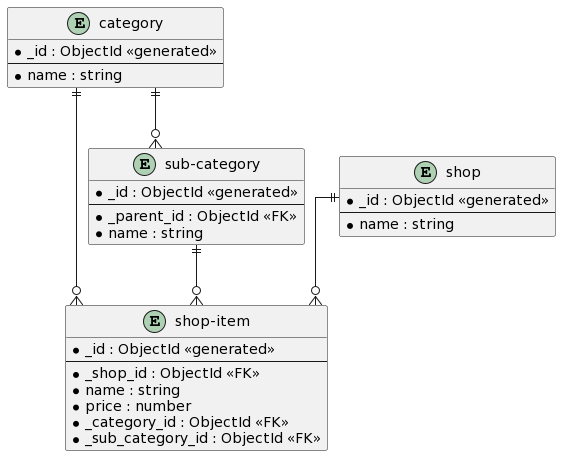
\includegraphics[width=0.85\linewidth]{img/shop_items_erd.png}
	\caption{Entity Relationship Diagram of Shop Item Data}
	\label{fig:serd}
\end{figure}

In conclusion, for large shop item data, MongoDB is flexible, fast, and scalable. The database schema meets the complex relationships between users, admins, categories, subcategories, shop items, and shops. It handles large amounts of data efficiently and adapts to e-commerce platforms. Thus, MongoDB is ideal for modern data management, especially for large, multifaceted datasets like shop items.

\newpage

\subsection{Application Programming Interface}

\subsubsection{Introduction}

When making modern software, the technology you use to build an Application Programming Interface (API) is very important. I chose to use ASP.NET Core along with the programming language C\# for the API part of my project. Several important factors, each of which added to the overall efficiency and reliability of the API, led to this decision.

One of the main reasons for choosing ASP.NET Core is that it works well with many NuGet packages. NuGet packages are basically code libraries or tools that are easy to add to a project. They provide a huge collection of resources that can improve functionality and speed up development. This wide range not only speeds up the development process but also gives you access to a lot of pre-built features, so you don't have to start from scratch.

Another big plus is that ASP.NET Core works natively with the Internet Information Services (IIS) server. This integration makes deployment and hosting easier, which guarantees strong performance and dependability. Its compatibility with MongoDB's driver makes it even more appealing, as it makes database interactions faster. Also, the fact that this framework has libraries for web scraping makes it easy to get data from different web sources, which is exactly what the project needs.
\newline\cite{aspnet}

The solution is designed so that the API is the central part of the application. It provides several features, like asynchronous web scraping, data manipulation, and providing important endpoints for both the web and mobile parts of the system. Also, it's an important security layer that handles how the applications and the database talk to each other, keeping the data safe and secure.

The authentication and authorization processes that the API handles add to the security by making sure that access to data and features is tightly controlled and in line with best practices. The Model-View-Controller (MVC) design pattern, which divides an app into three parts that are all connected, forms the basis of the API's structure. This not only makes the code cleaner and easier to maintain, but it also helps separate concerns, which makes the system more modular and scalable.

One interesting thing about the API is that it uses OpenAI to process and organize data that it gets from web scraping. As a result of this integration, the API can do more than just handle data. It's an innovative combination of traditional web development methods and artificial intelligence technologies.

\newpage

To sum up, the decision to use ASP.NET Core with C\# for the API is a smart move that takes advantage of a strong, flexible, and effective technology stack. It's made to handle the application's complicated needs, giving a solid base for working with data, keeping it safe, and making it easy to connect to other parts of the system.

\noindent\textbf{Structure of the API}

\subsubsection{Entry Point}

The setup process revolves around \textbf{WebApplicationBuilder}. This builder lets developers configure app services and settings. CORS policies instruct the web app how to handle requests from different domains. This is crucial for modern web apps that use resources or APIs from different domains to ensure safety and functionality. Configuration includes database service setup. User model, shop item, shop item category, and shop scraping services are added as singletons, meaning they are used once throughout the application.

The code also configures JWT authentication. This is crucial to modern web apps because it restricts access to resources and endpoints to verified users. This app uses these tokens to verify users' identities and manage them well, such as by getting them from cookies.

The final step is building the app and setting up its middleware pipeline. This pipeline manages HTTP requests, CORS, authentication, and controller requests. Controllers require a RESTful API design with multiple endpoints for different web requests. After saving the settings, the app can be launched and serve requests as a web server.

\subsubsection{Controller}

The \textbf{DataBaseService} is an important part of the proposed system architecture. It acts as a flexible data service with generic datatype of for the model. This helps with the developer as creating a new controller is relatively easy, promoting high flexibility for future changes. It manages the flow of information between the controllers and the MongoDB driver.  

The ASP.NET Core \textbf{ControllerBase} class is at the heart of this structure, and an ApiControllerBase class is carefully built on top of it. Its design is naturally generic, which makes it useful because it can be used as a base for building different kinds of controllers that are each made to work with specific models, therefore promoting scalability.

In addition to managing a lot of asynchronous methods related to data manipulation, this derived class is also in charge of managing JWT tokens within cookies crucial to the security of the endpoints. The 'AllowAnonymous' attribute on the HTTP method in the derived controller can selectively bypass JWT authentication.

The architecture also includes the \textbf{ShopItemController} and \textbf{ShopItemCategoryController}, which are both used to change the general properties of their own data types. This controller is used by, the mobile application to retrieve data and the scraping service to expand, update the data warehouse.

The \textbf{UserController} is the most complicated of these. Its job is to handle a wide range of user-related tasks. These include creating and deleting user accounts, logging in and out, authenticating users, verification of administrative privileges, assigning admin rights, and renewing refresh tokens that have expired.

Shown below is a detailed class diagram so that one can fully understand how the different parts of this system work together. Figure \ref{fig:ccd} shows very clearly how different classes and interfaces are linked to each other, along with their properties and methods.

\begin{figure}[H]
	\centering
	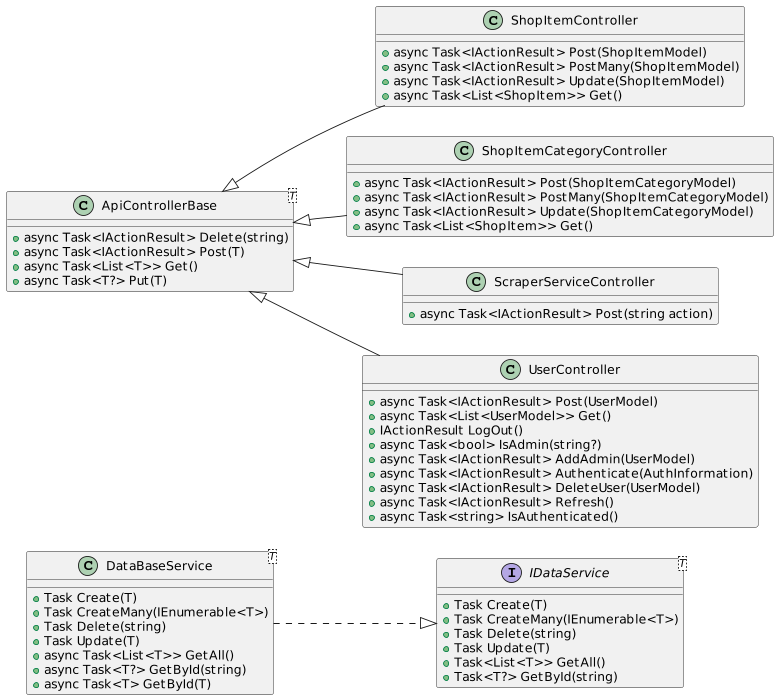
\includegraphics[width=1\linewidth]{img/controller_classdiagram.png}
	\caption{Class Diagrams Related to the Controller}
	\label{fig:ccd}
\end{figure}

\newpage

\noindent\textbf{UserController in Detail}

Since UserController is a complex part of the application, mostly because that is how it handles authentication, it is useful to talk about the implementation a little more in detail.

\begin{figure}[H]
	\centering
	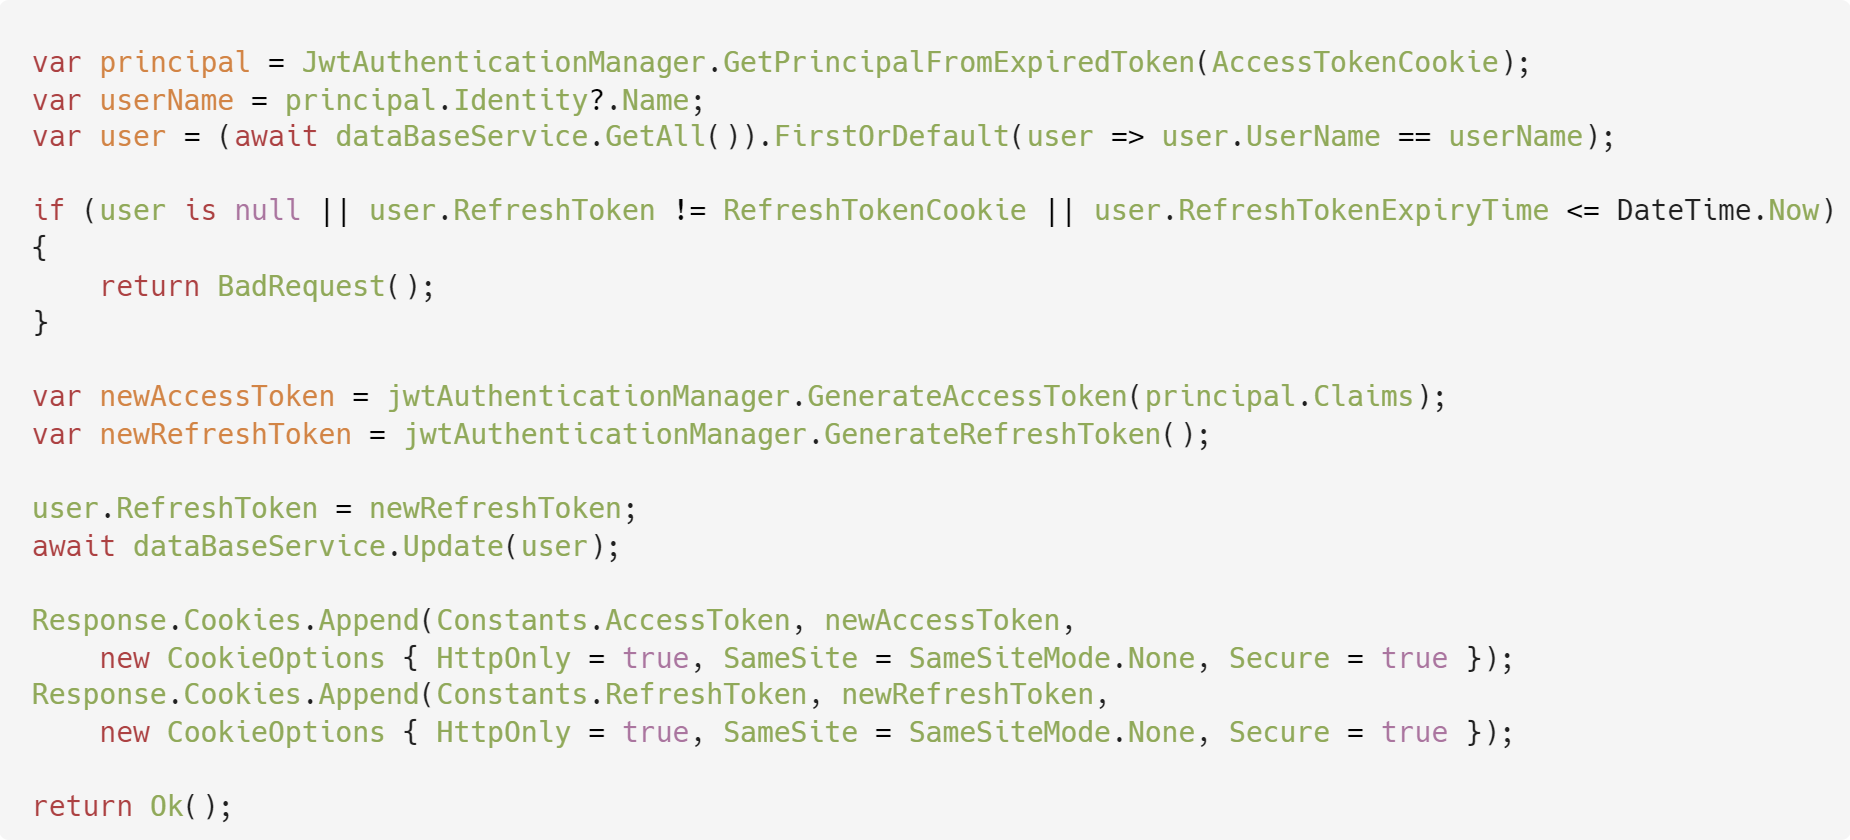
\includegraphics[width=1\linewidth]{img/code_auth.png}
	\caption{Authentication Snippet}
	\label{fig:authcode}
\end{figure}

In the provided snippet the authentication process is visible, with an additional JWT token refresh process, which is only needed if at the time of the request, the token of the user was expired, in which case, the system checks whether or not the user's other information and additional token is valid, in which case it generates a net token, which the user can use for authentication.

Upon registering, the user's provided password is immediately hashed and only stored afterwards, and in every login process the hashed passwords are being matched to each other.
On logging out, the system removes all the cookies from the user, which is achieved by setting the cookies expiration date to a value, which will essentially turn them invalid.

Regarding the addition of a new admin user, the process will only be successful when the user assigning admin role to another user has admin privileges. More on the authentication process, with detailing the JWT authentication process will be discussed in the next section.

\subsubsection{JWT Authentication}

The authentication for the web uses JSON Web Tokens and takes advantage of AspNetCore's Authentication libarary, as well as the IdentityModels's Jwt token library. JSON Web Tokens (JWTs) are compact, URL-safe claims that are used for secure authentication and information exchange in web applications.

\begin{figure}[H]
	\centering
	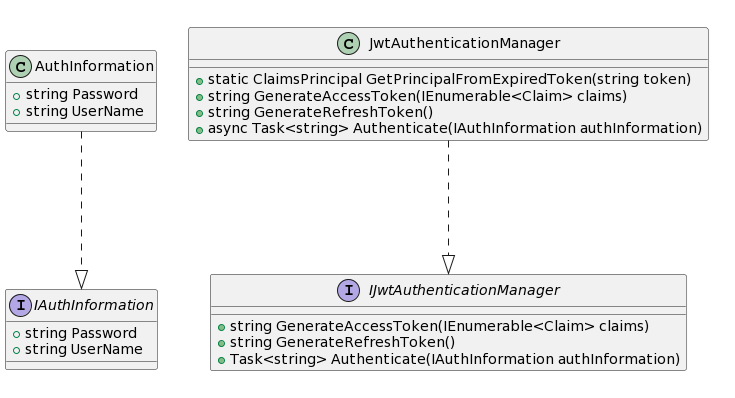
\includegraphics[width=0.8\linewidth]{img/authentication_classdiagram.png}
	\caption{Class Diagrams Related to JWT Authentication}
	\label{fig:acd}
\end{figure}

Figure \ref{fig:acd} represents the class for holding authentication information as well as the authentication manager class which is responsible for handling all JWT authentication related tasks. The implementation of the class is explained on the next page and represented by the following code snippet:

 \begin{figure}[H]
 	\centering
 	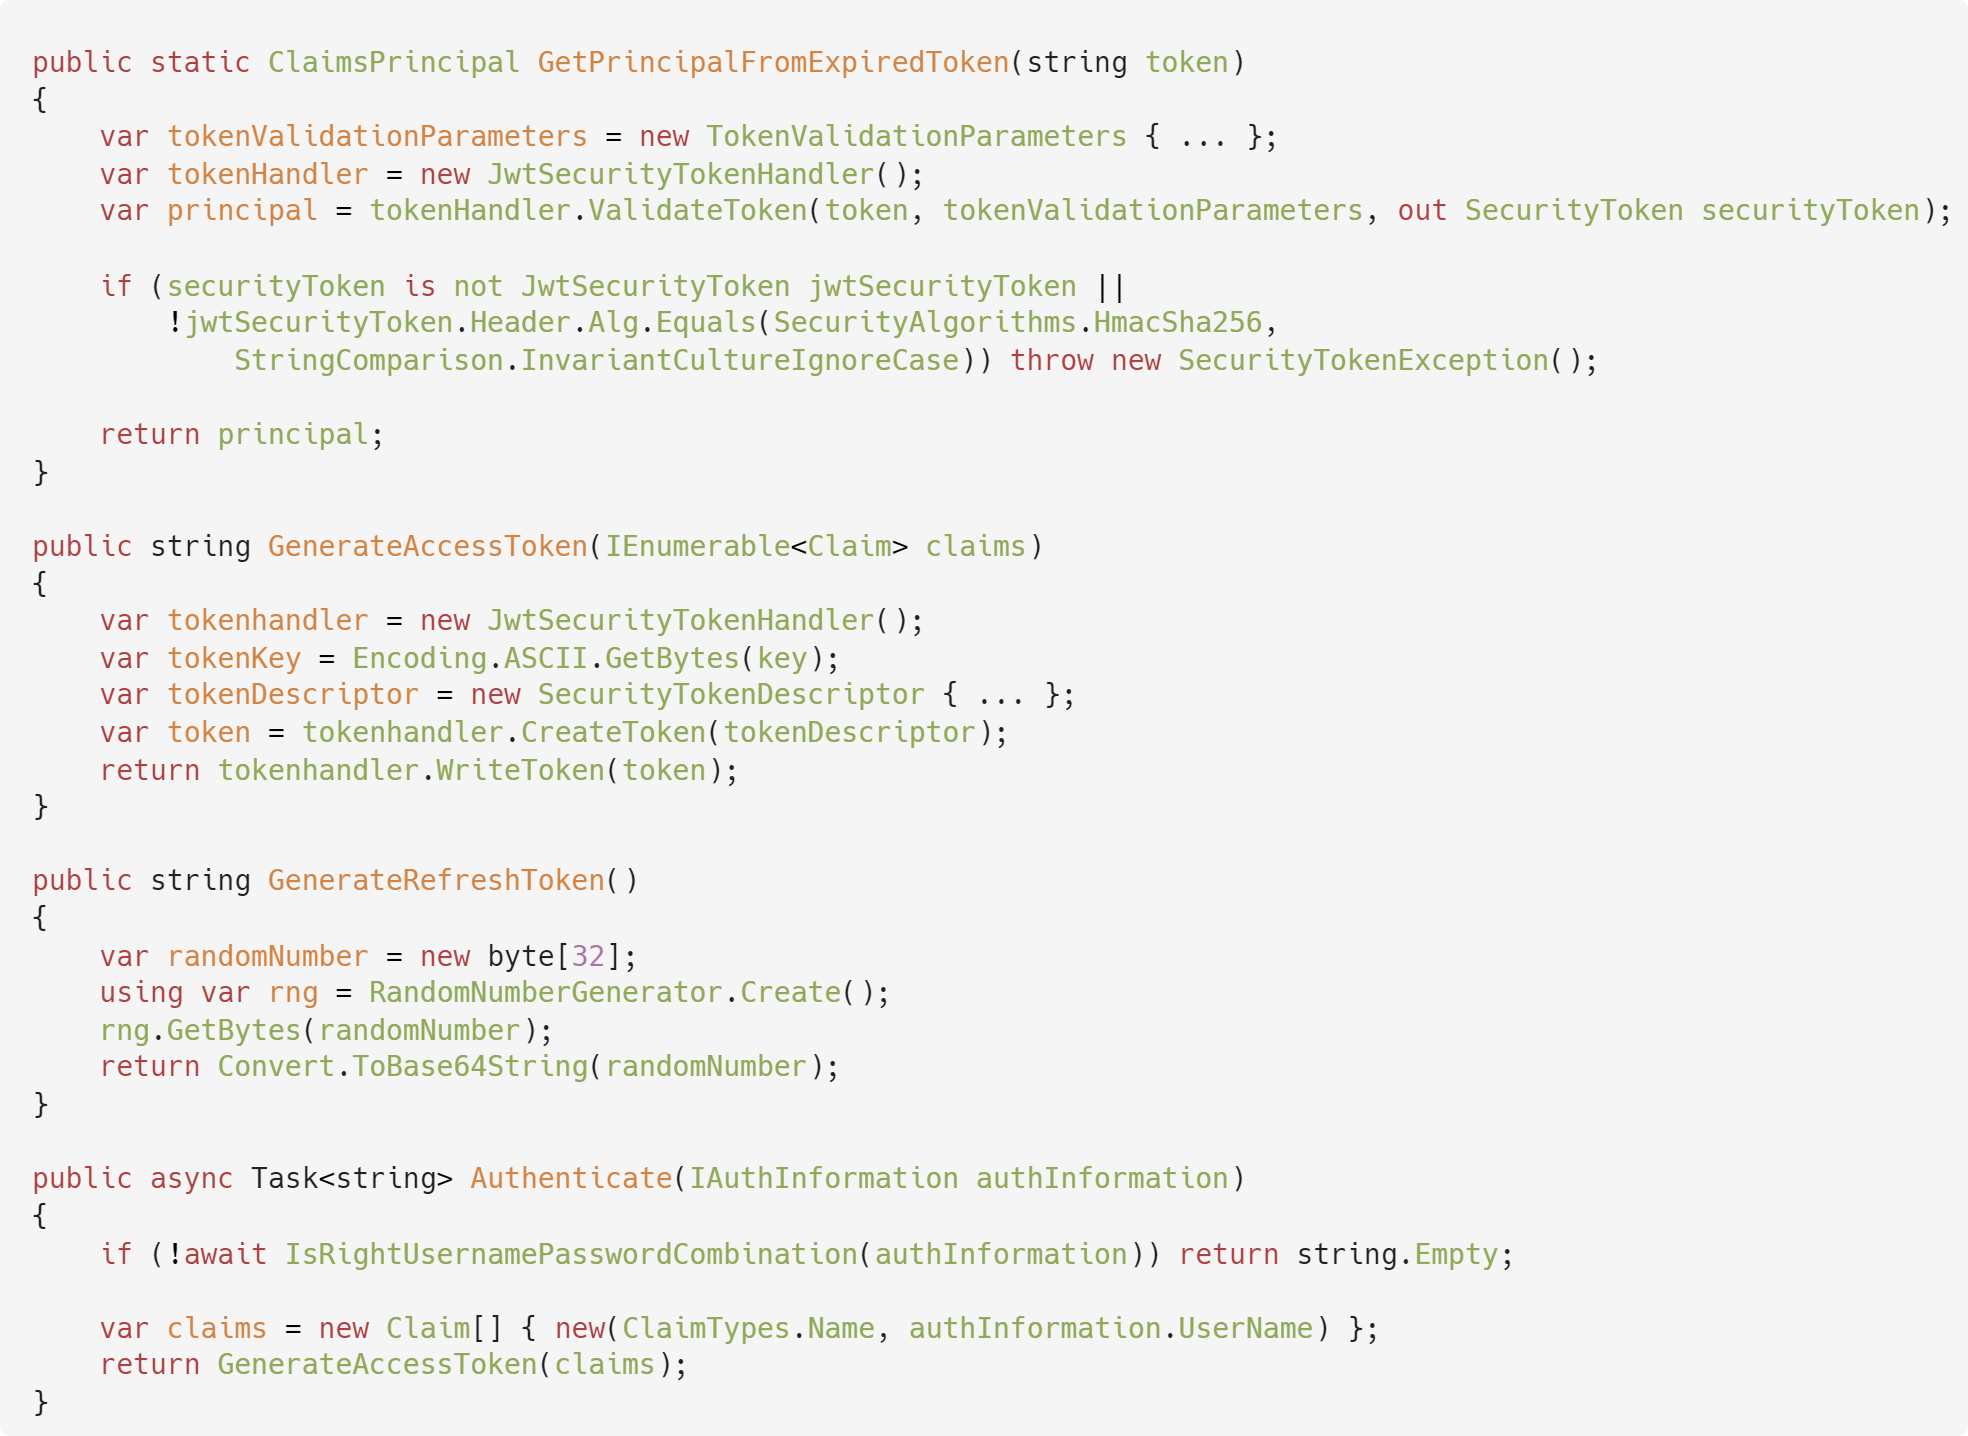
\includegraphics[width=1\linewidth]{img/code_jwt.png}
 	\caption{Authentication Snippet}
 	\label{fig:jwtcode}
 \end{figure}
 
\textbf{ GetPrincipalFromExpiredToken(string token):} This function throws an exception if the token is invalid or not in the expected format and verifies an expired JWT token in order to extract and return its ClaimsPrincipal.
 
\textbf{ GenerateAccessToken(IEnumerable<Claim> claims):} With the supplied claims, it generates and returns a new JWT access token.
 
\textbf{ GenerateRefreshToken():} creates a base64 string that can be used as a refresh token by randomly selecting a 32-byte number.
 
\textbf{ Authenticate(IAuthInformation authInformation):} This function verifies a user's identity using the credentials they have provided. If successful, it returns a new JWT access token; otherwise, it returns an empty string.
 
\subsubsection{Data Models}

While being an essential part of the MVC pattern, the  data models in the application are mostly used for data representation, and moving data in a structured way between the API endpoints and the database. Only the UserModel includes specific methods for password hashing and verifying using \textbf{BCrypt.Net-Next library's} \textit{EnhancedVerify()} method, that checks a plaintext password against a hashed version to ensure secure authentication as well as \textit{EnhancedHashPassword()} method, that uses bcrypt hashing algorithm and other security enhancements to make storing passwords secure. The structure of the data models used by the controllers as well as showcasing how easily extensible the genereic controller implementation is shown on the figure \ref{fig:dcd}.

\begin{figure}[H]
	\centering
	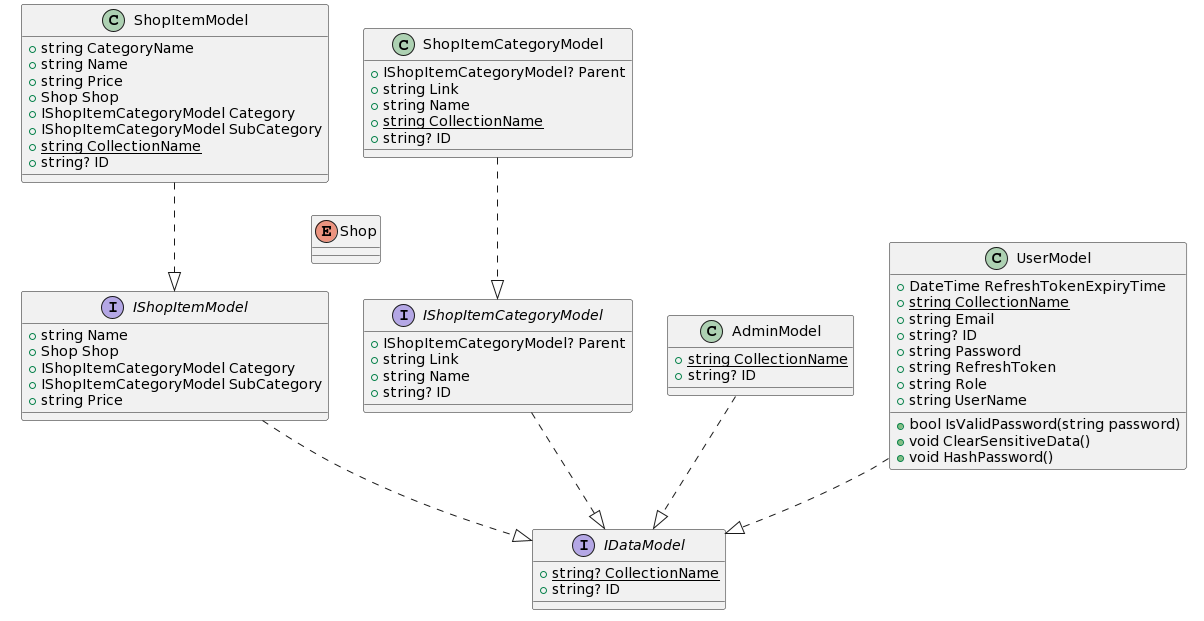
\includegraphics[width=1\linewidth]{img/datamodel_classdiagram.png}
	\caption{Class Diagrams Related to Data Models}
	\label{fig:dcd}
\end{figure}

\newpage

\subsubsection{Web Scraping}
In the solution the API is responsible for handling the data collection from the web as well. The scraping service is accessible from the website on a specific page available for administrators only, where they can force an immediate process or set a time interval for automatic executions. For crawling the web the solution uses a version of Selenium framework provided for .Net applications.

\textbf{Selenium} is a free and open-source automation tool that is mostly used to automate web browsers. It gives engineers a solid way to check web applications. Many people choose Selenium for cross-browser automation for it has many useful parts, such as Selenium WebDriver for managing how browsers work, which is crucial in this case.

The first approach consisted of downloading the page's HTML code, however it turned out that nowadays most of the websites load content dynamically, so the data downloaded was of no use. To overcome this, the application uses Selenium for simulating a head-less browser, which is a web browser that doesn't have a graphical user interface. It lets programs control web pages automatically, which is why it's often used for web scraping, automated testing, and rendering web pages for processing on the server.

Scraping also states an issue with protection of the site's data. The general rule is that you are only supposed to collect data, that you can publicly access and if the site's robots.txt file content does not prohibit you from scraping the data available on the website. Before crawling a new website for data, it is essential to review these points.

Shown below on figure \ref{fig:scd} are the classes and interfaces that are required for the service to work, the characteristics of its working process are explained on the next page.

\begin{figure}[H]
	\centering
	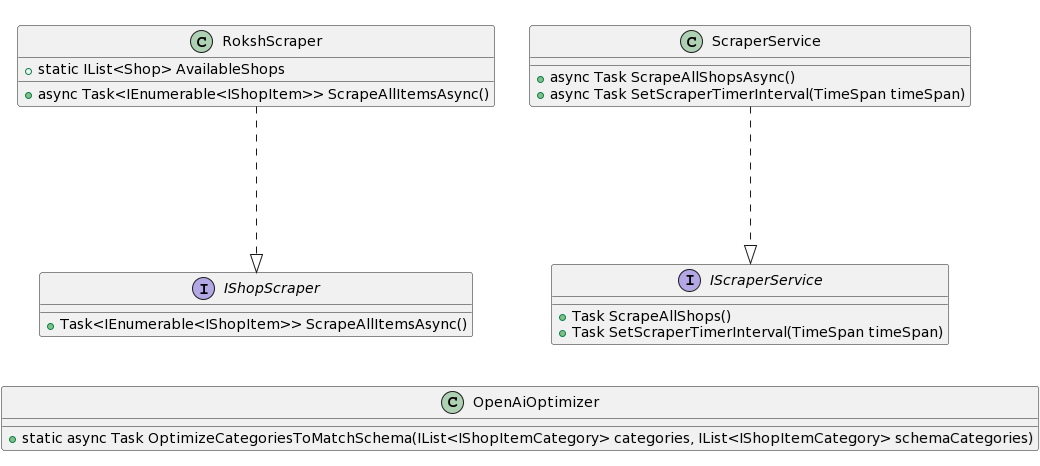
\includegraphics[width=1\linewidth]{img/scraping_classdiagram.png}
	\caption{Class Diagrams Related to Web Scraping}
	\label{fig:scd}
\end{figure}

\noindent\textbf{How Does It Scrape}

First of all, the ScraperService is exported as a singleton IScraperService during the application setup process. The ScrapeServiceEndpoint listens for post requests, and upon a valid request takes action. It is configured to allow requests for immediate and timed scrapings. 

Before scraping, the service configures the parameters for the WebDriver and calls for all of the available IShopScraper implementations. Since many websites differ in their structure, most of them need separate implementations to specify what instructions are required for the data retrieval. 

After finishing the setup, the service starts all of the IShopScrapers data collection processes on different threads to speed up the process, then waits for all of them to finish. On finishing it checks the integrity of the data, using fuzzy string matching and uploads the data into the database.

The process of scraping the items from various websites always needs fine tuning, but roughly follows the same idea implementing HTML and CSS tag verification, which will be presented with the following four pseudo-like algorithm descriptions.


\noindent\textbf{ScrapeAllItemsAsync Method} is the one being called from the Service and in the end provides structured shop item data with correct categories provided by the application.

\noindent\textbf{GetCategoriesWithSubcategories Method} is the one responsible for mapping all categories and subcategories on the site with storing their links to easily load when needed.

\noindent\textbf{ScrapeShopItemsAsync Method} visits every subcategory and scrapes all the items that are available on that page, then stores them for later use.

\noindent\textbf{ScrollTillEnd Method} is crucial for the scraping process, since it handles the scrolling and waiting process, to make sure that the dynamically loading item data is present and scrapable.

\begin{algorithm}
	\caption{ScrapeAllItemsAsync Method}
	\begin{algorithmic}
		\State $attempts \gets 0$
		\State $maxAttempts \gets 3$
		\While{$attempts < maxAttempts$}
		\State \textbf{try to}:
		\State \hspace{\algorithmicindent} $items \gets \text{ScrapeShopItemsAsync().ToList()}$
		\State \hspace{\algorithmicindent} $\text{webDriver.Quit()}$
		\State \hspace{\algorithmicindent}\hspace{\algorithmicindent} $\text{OpenAiOptimizer.}$
		\Statex \hspace{\algorithmicindent}\hspace{\algorithmicindent} \hspace{\algorithmicindent} $\text{OptimizeCategoriesToMatchSchema(allCategories, defaultCategories)}$
		\State \hspace{\algorithmicindent} \Return $items$
		\State \textbf{if} exception occurs \textbf{then}
		\State \hspace{\algorithmicindent} $attempts \gets attempts + 1$
		\State \hspace{\algorithmicindent} \textbf{if} $attempts > maxAttempts$ \textbf{then}
		\State \hspace{\algorithmicindent}\hspace{\algorithmicindent} Print exception $e$
		\State \hspace{\algorithmicindent}\hspace{\algorithmicindent} \textbf{break}
		\EndWhile
		\newline
		\Return new list of IShopItem
	\end{algorithmic}
\end{algorithm}

\vspace{-500pt}

\begin{algorithm}
	\caption{GetCategoriesWithSubcategories Method}
	\begin{algorithmic}
		\State Initialize dictionary $categoriesWithSubCategories$
		\State Create a new WebDriverWait with 5 seconds timeout
		\For{each category element found by webDriver}
		\State Click on the category element
		\State Create a ShopItemCategory
		\State Initialize list for $subCategories$
		\For{each subCategory in the category element's parent}
		\State Add new ShopItemCategory to $subCategories$
		\EndFor
		\If{no $subCategories$}
		\State Add the main category as a subcategory
		\EndIf
		\State Add category and its $subCategories$ to the dictionary
		\EndFor
		\newline
		\Return dictionary
	\end{algorithmic}
\end{algorithm}

\begin{algorithm}
	\caption{ScrapeShopItemsAsync Method}
	\begin{algorithmic}
		\State Navigate webDriver to URL
		\State Initialize list of IShopItem $items$
		\For{each category in GetCategoriesWithSubcategories}
		\For{each subCategory in category's value}
		\State Add $subCategory$ to allCategories
		\State Navigate webDriver to $subCategory$'s link
		\State Call ScrollTillEnd
		\For{each item found by webDriver}
		\State Create and add new ShopItem to $items$
		\EndFor
		\EndFor
		\EndFor
		\newline
		\Return $items$
	\end{algorithmic}
\end{algorithm}

\begin{algorithm}
	\caption{ScrollTillEnd Method}
	\begin{algorithmic}
		\State Initialize $endOfPage \gets false$
		\State Create a new WebDriverWait with 5 seconds timeout
		\While{not $endOfPage$}
		\State Get count of items found by webDriver
		\State Scroll to the end of the page
		\State \textbf{try to}:
		\State \hspace{\algorithmicindent} Wait until more items are found
		\State \textbf{if} exception occurs \textbf{then}
		\State \hspace{\algorithmicindent} Set $endOfPage \gets true$
		\EndWhile
	\end{algorithmic}
\end{algorithm}

\newpage

\subsubsection{OpenAI Processing}

Unfortunately it can't be guaranteed that each site has the same categories for the products listed, therefore I needed a solution to match these. Fuzzy string matching would not be reliable enough, therefore I turned to OpenAI's chat endpoint and utilized it the following was: Before returning the data to the ScrapingService, the IShopScraper calls of the OpenAiOptimizer's OptimizeCategoriesToMatchSchema method.

A system calls the OptimizeCategoriesToMatchSchema method to divide categories into 10 groups and asynchronously send them to OpenAI's ChatGPT as JSON data. ChatGPT matches these categories to a schema and returns renamed JSON categories. After renaming the categories, the method returns the modified data to the calling system. This way AI-driven classification and automated data processing are also shown in this web application.

Interesting remark about the prompting process, is that it is not included in a ChatGPT subscription, instead it uses a credit / prompt system, which has become much cheaper, since the introduction of the GPT 3.5 turbo model. The code also needs to be prepared for occasional outages, when it needs to retry the prompt. Writing a message with instructions for ChatGPT can be challenging too, I overcame this by writing a sturdy prompt message and asking ChatGPT to reply with a JSON format of the data. This sometimes also produced extra message and characters around the JSON format, which I worked around by trimming all the characters, outside the JSON body format. On figure \ref{fig:ai} a simplified version of the process is shown via sequence diagram.

\begin{figure}[H]
	\centering
	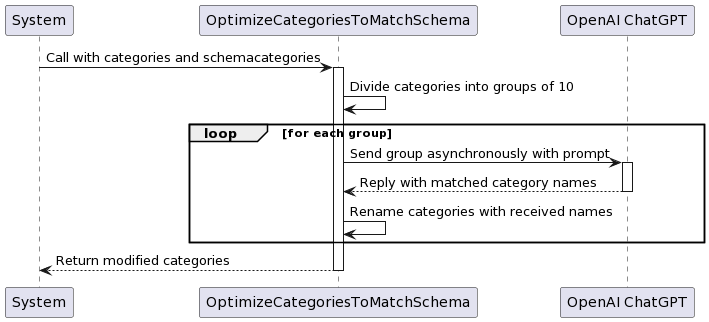
\includegraphics[width=1\linewidth]{img/openai_sequence.png}
	\caption{Open AI Category Aligning Sequence Diagram}
	\label{fig:ai}
\end{figure}

\pagebreak

\subsection{Web Application}

\noindent\textbf{Who is it for?} It is very important to note, that the web application is solely for administration purposes and will only be accessible by the program's administrators and the associated retailers to provide them a way to upload their product data. In this section by users I essentially mean one of the retailers who are providing data for the application.

\subsubsection{Introduction}

As the framework of choice for this app, Angular was chosen because it has a large ecosystem and a lot of strong features that make it perfect for a modern, dynamic web app.

As a platform known for its structured framework and wide range of tools, Angular makes it easy to build large-scale apps with its opinionated architecture. This prescriptive nature makes it much easier to keep codebases consistent, which makes it perfect for the application's complicated structure, which needs clear modularity and separation of concerns.

Angular's powerful typing system, which is powered by TypeScript, makes code better and more reliable. This makes debugging and maintenance easier, which is important for the long-term growth and scalability of the app. Using reactive programming patterns with RxJS also makes it easier to work with asynchronous data streams, which are needed for the app's real-time data processing features like uploading product data and scraping the web.

Built-in features of the framework, like dependency injection, routing, and services, make it easier to make applications that are safe and work well. The app uses these features to keep track of user authentication states, protect routes based on user roles, block HTTP requests, and easily talk to back-end services. Moreover the architecture carefully arranges how users interact with it, how it is protected, and how it handles data through a clear set of modules.
\newline\cite{angular}

By implementing SSL certificates for the web page and API, the application enables HTTPS protocol and ensures secure communication. Sensitive data, including passwords and tokens, is protected by this configuration, which encrypts data transferred between the server and client. By using HTTPS instead of HTTP, users can be assured that their data is encrypted and unintelligible even if it is intercepted, creating a secure and reliable environment. The application's design is based on this commitment to security, and it fits in perfectly with Angular's framework, which facilitates strong security implementations.

\newpage

\subsubsection{Architecture}

The following diagram, visible on figure \ref{fig:webappstruct} makes it easy to see how the application is structured. Every module makes sure that the user has a safe, quick, and smooth experience by explaining its function in the application and how it works with the other modules. This organized method makes things run more smoothly and sets the stage for future improvements.

\begin{figure}[H]
	\centering
	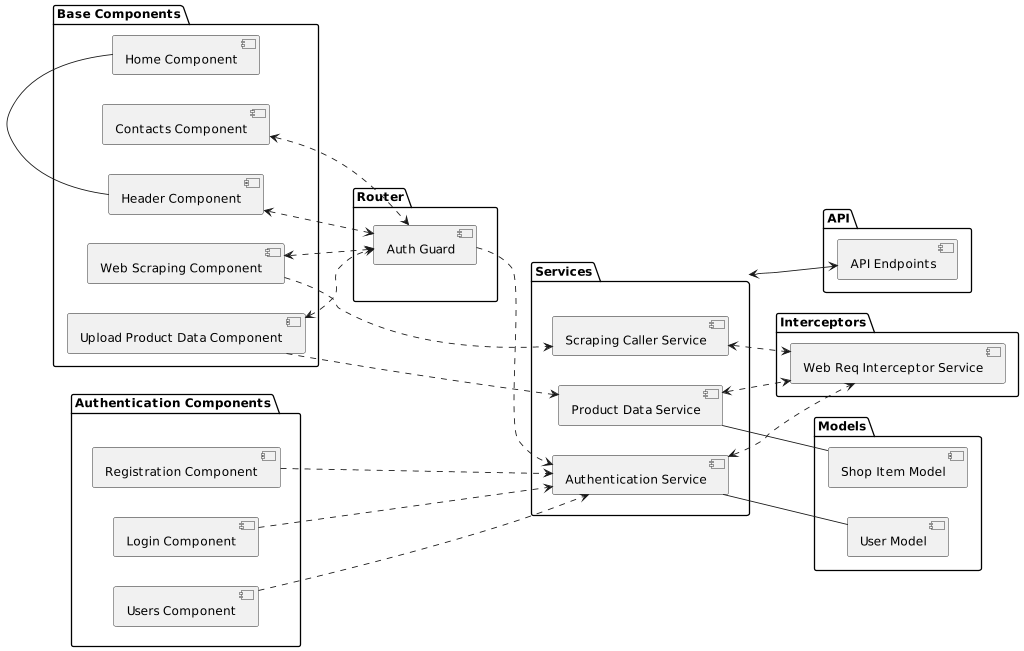
\includegraphics[width=1\linewidth]{img/website_structure.png}
	\caption{Structure of the Web Application}
	\label{fig:webappstruct}
\end{figure}

\noindent\textbf{Base Components: }

The Base Components make up the main part of the user interface. The Home Component is a landing page with useful information that all visitors can see. The Header Component goes with it and makes sure that the application's navigation and branding are all the same. The header navigation depends on whether a user is authenticated or not as well as if they have admin privileges or not. 

\noindent\textbf{Authentication Components:}

It essentially includes two main parts: the Registration Component, which lets new users create accounts, and the Login Component, which helps users prove who they are. Both parts are necessary to start the user's journey within the app by giving them JWT access and refresh tokens when they successfully register or login.

On figure \ref{fig:auth} the UI of the two authentication components, login and registration functionalities are visible. 

\begin{figure}[H]
	\centering
	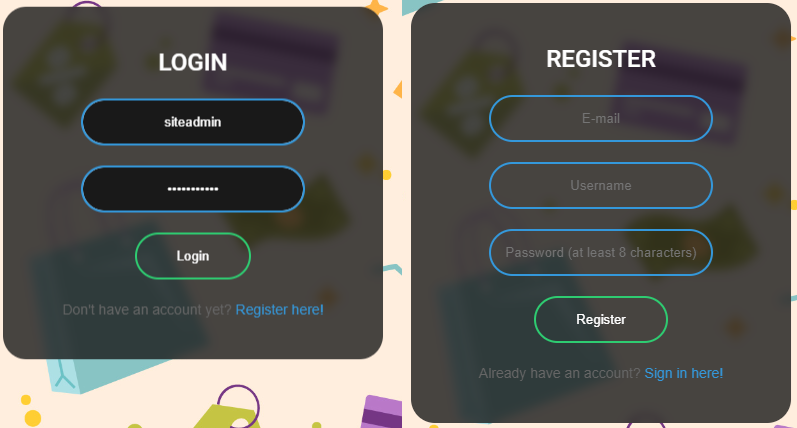
\includegraphics[width=0.7\linewidth]{img/auth_web_ss.png}
	\caption{Authentication on the Website}
	\label{fig:auth}
\end{figure}

\noindent\textbf{Specialized Access:}

Two essential components—the Web Scraping Component and the Users Component—are only accessible to admin users. With the former, administrators can set up and start web scraping activities on demand or at predetermined intervals, which functions are provided with an easy to use user interface shown on figure\ref{fig:webcrapingreq}.
\begin{figure}[H]
	\centering
	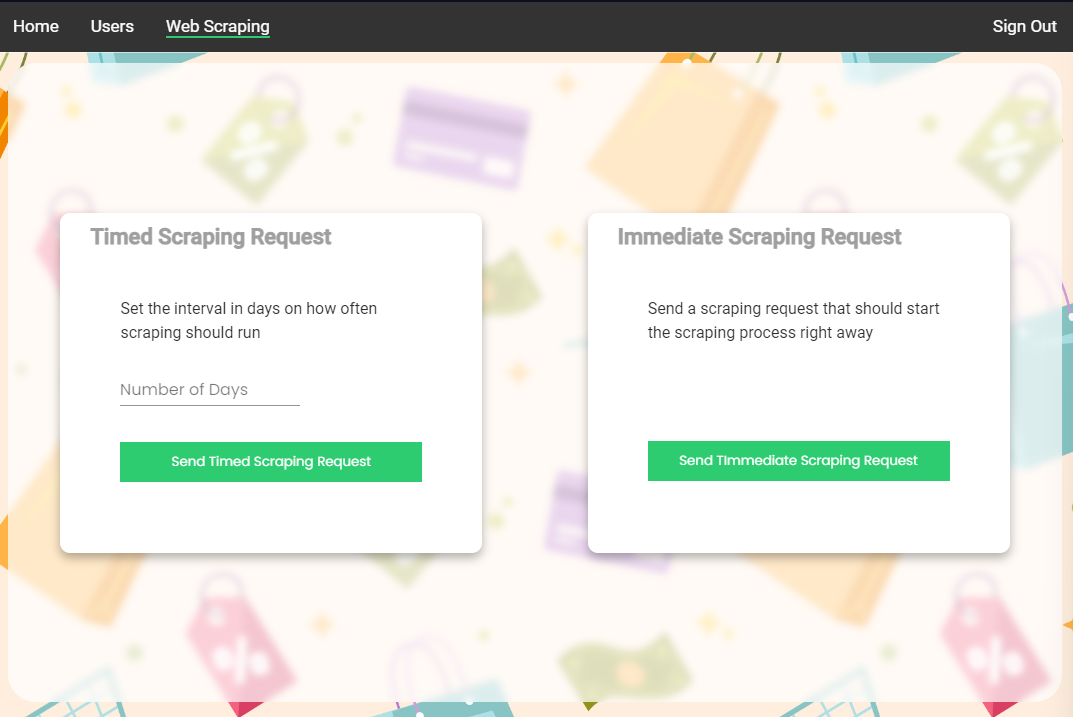
\includegraphics[width=0.9\linewidth]{img/scraping_web_ss.png}
	\caption{Requesting Web Scraping}
	\label{fig:webcrapingreq}
\end{figure}

\newpage

With utilizing the Users Component, the administrators can view a complete list of users available for the web application, change their permissions within the application or completely remove them from the list. The interface for these functions are shown on figure \ref{fig:umgmt} below.

\begin{figure}[H]
	\centering
	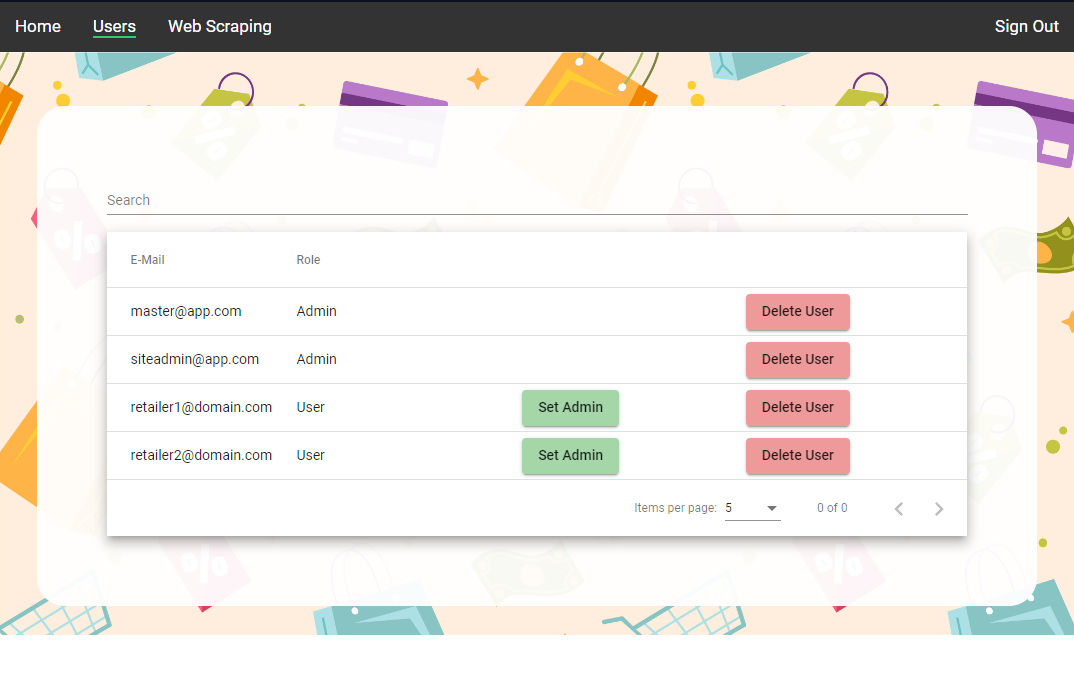
\includegraphics[width=0.8\linewidth]{img/users_ss.png}
	\caption{Web Application's User Management}
	\label{fig:umgmt}
\end{figure}

\noindent\textbf{User-Focused Functionality:}

Authorized users are given permission to access the Contacts Component for the purpose of communication and the Upload Product Data Component. The latter component, shown on figure \ref{fig:uploaddata} is provided for users to upload product data, which is then processed by the Product Data Service, which converts CSV inputs into JSON format and checks that they match the Shop Item Model before submitting them to the API.

\begin{figure}[H]
	\centering
	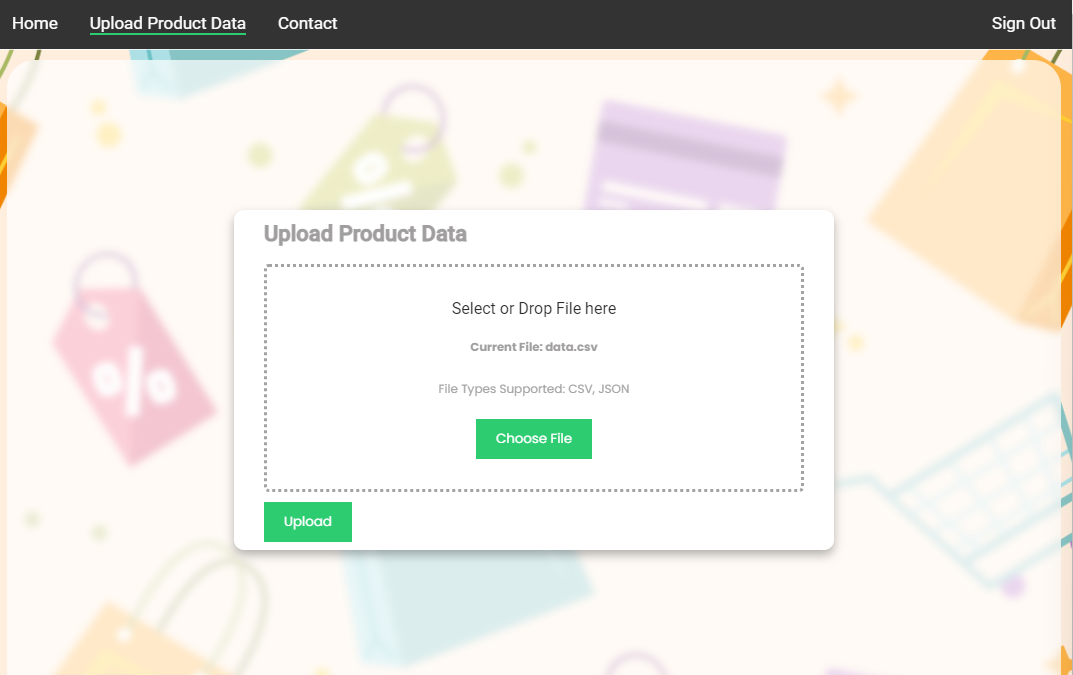
\includegraphics[width=0.65\linewidth]{img/product_data_ss.png}
	\caption{Upload Product Data}
	\label{fig:uploaddata}
\end{figure}

\noindent\textbf{Services:} 

The logic of the application is contained within the Services, which includes the Product Data Service, Authentication Service, and Scraping Caller Service. To fulfill specific application functionalities, each service interacts with the corresponding components and API Endpoints.

\noindent\textbf{Data Models:} 

The User Model and the Shop Item Model define the structure for user information and product data. These models are critical for the application's data integrity and consistency.

\noindent\textbf{Interceptors:} 

All outgoing requests are carefully watched over by the Web Req Interceptor Service. It makes sure that authentication keeps going by refreshing tokens (visible on figure \ref{fig:cookies}) through the Authentication Service when needed and stopping requests and logging out the user if serious problems are found.

\begin{figure}[H]
	\centering
	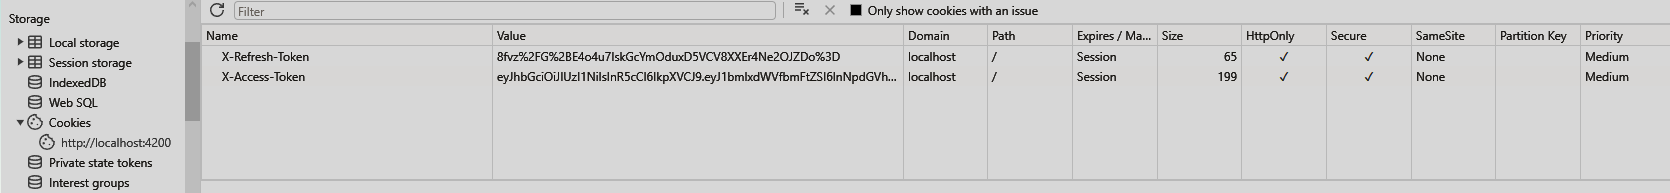
\includegraphics[width=1\linewidth]{img/cookies_ss.png}
	\caption{JWT Tokens Stored in Cookies}
	\label{fig:cookies}
\end{figure}


\noindent\textbf{Router:} 

The Router and Auth Guard are essential to the application's security architecture. It ensures that non-authenticated users can only access the Home, Registration, and Login Components by clearly defining user interfaces and component accessibility. Admins and verified users, on the other hand, have access to extra, role-specific features.

\noindent\textbf{API Communication:}

Backend interaction happens through the API package. The document defines the endpoints that the application uses to talk to the backend, trusting the Services to do all of those tasks efficiently.

\noindent\textbf{Ending Note:}

Even though that the web application only serves administrative purposes, it was still important to provide this functionality in a user friendly manner. From development side, since the future is malleable choosing Angular was the right way to ensure modularity and scalability. 

\newpage

\subsection{Mobile Application}

\subsubsection{Introduction}

The following chapter of this thesis discusses the mobile application I created using the .NET MAUI framework. .NET MAUI is a modern cross-platform development tool that enables applications to be easily adapted to a variety of operating systems, including Android, iOS, TizenOS, and macOS. I used several NuGet packages during the application's development, which significantly increased functionality and user experience. These packages include CommunityToolkit.Maui, which supports specific user interface elements, FuzzySharp, which enables fuzzy search based on product names, and ZXing.Net.Maui, which helps with barcode reading and decoding.

During the project's development, I used the MVVM (Model-View-ViewModel) design pattern, which is a common architectural pattern in modern application development. The benefit of MVVM is that it effectively separates the user interface (View), data model (Model), and presentation logic (ViewModel). This separation simplifies the development process by allowing components to be tested and maintained more easily. The ViewModel serves as an intermediary between the model and the view, reducing direct dependencies and increasing the application's flexibility, making it easier for developers to manage business logic and user interface.
\newline\cite{maui}

The current application can be compared to a Minimum Viable Product (MVP), as it demonstrates basic functionality and serves as a solid foundation for future development. The MVP approach allows for the collection of user feedback in the early stages of a project, which can then be used to better determine future development directions. The scope of the project is extensive, and many ideas have yet to be implemented. In the field of software development, it is common to adapt and redesign in comparison to the original plans, which is difficult, but the MVP approach used allows the application to gradually develop further, achieving a balance between user needs and project framework. \cite{mvp}

In the following sections, I will discuss the architecture of the application, the persistence of data, I will highlight some interesting solutions that have been implemented, and I will provide an overall general idea of how the application functions.

\pagebreak

\subsubsection{Service Layer}

\begin{figure}[H]
	\centering
	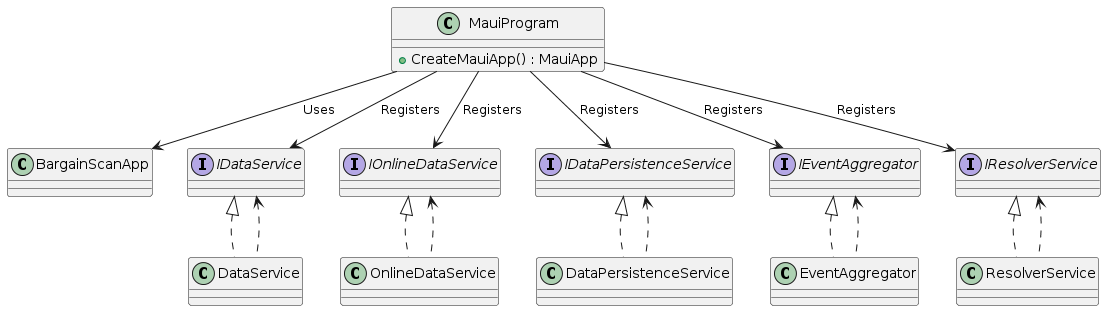
\includegraphics[width=1\linewidth]{img/app_services.png}
	\caption{Mobile App Services}
	\label{fig:appservices}
\end{figure}

Visible on figure \ref{fig:appservices}, the MauiProgram is the application's entry point, and it properly builds the BargainScanApp by injecting all of the required services into the dependency injection container. These services are required for the application to function properly while adhering to the key MVVM principles.

\noindent\textbf{ResolverService}

The ResolverService in automatically links Views to the ViewModels that go with them. It uses a naming convention where the ViewModel is called the same thing as the View, but with "Model" added at the end.

This service is registered with the dependency injection container, just like any other service. All classes that end in "View" or "ViewModel" are looked for in the app. It finds the ViewModel that goes with each View and registers a factory method that makes the View and sets its DataContext to a ViewModel instance.

With this method, setting the DataContext for a View is done automatically, so modules don't have to care for it. There is a separation of concerns with this approach, as Views are not connected to the creation and retrieval of their ViewModels.

\noindent\textbf{EventAggregator}

The EventAggregator is a communication mechanism that enables loosely coupled interactions between application components. It includes Publish, Subscribe, and UnSubscribe methods that allow components to communicate without using direct references.

In the MVVM pattern, the EventAggregator replaces standard .NET events to reduce coupling and improve modularity. It enables components to communicate without knowing each other, thereby increasing reusability and testability. This is especially important in MVVM, where separation of concerns and loose coupling are fundamental principles.

\noindent\textbf{OnlineDataService and DataPersistenceService}

It is the OnlineDataService's responsibility to communicate with the API; however, it is only used when the application lacks data or has outdated data about the products contained in the API. The DataPersistenceService is used to load and save retrieved shop items, the local user profile, the user's registered shopping carts, and descriptive information.

\noindent\textbf{DataService}

\begin{figure}[H]
	\centering
	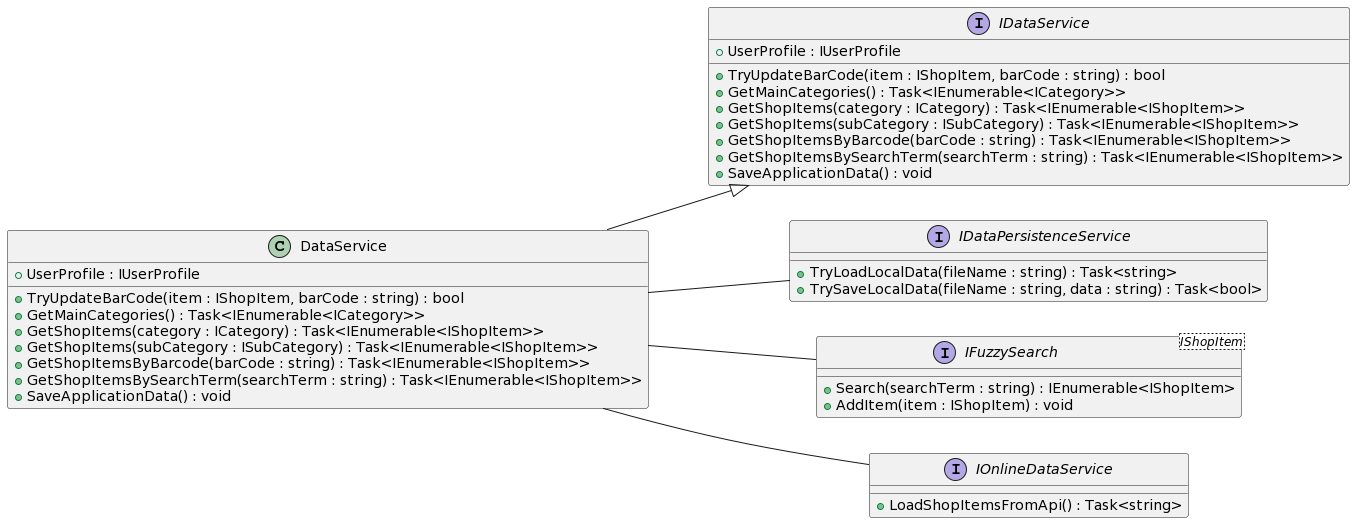
\includegraphics[width=1\linewidth]{img/app_dataservice.png}
	\caption{Mobile App DataService}
	\label{fig:appdataservice}
\end{figure}

The \textbf{DataService}, visible on figure \ref{fig:appdataservice}, is the primary service that allows users to access and manipulate application data across the entirety of the application. It makes use of IDataPersistenceService for the purpose of saving and loading local data, and it makes use of IOnlineDataService for the purpose of accessing data from the API. 

It is responsible for implementing the IDataService interface, which defines the methods that the service offers. Through the process of build-up, the service is injected into the application, which guarantees that it will be accessible throughout the entirety of the runtime. It is possible to execute the majority of the DataService's methods in an asynchronous manner, which guarantees that the user interface will not become unresponsive in situations where a lot of computational power is required. 

The modules that make use of it are able to access shop items classified into particular categories or subcategories, as well as search for those items using barcodes or search terms, with the latter method employing fuzzy string matching for improved performance. It also manages the process of assigning a barcode to a product in the event that the product has not yet been assigned with a barcode. 

\pagebreak

The service is also in charge of handling data for the local user profile, managing registered shopping carts, determining which shopping cart is active, and allowing the metadata and content of the shopping carts to be modified.

Additionally, it offers a method for saving application data on the fly, and it is responsible for loading information from either local or online sources when the application is started up. It is important to note that the data that is saved locally is saved in the data folder of the application using the JSON format. This ensures that the data is secure and invisible to any malicious attempts. 

\noindent\textbf{FuzzySearch}

As part of DataService a generic class called FuzzySearch is used to perform fuzzy searches on a group of objects of type T that implement the INamed interface. Similarity scores are computed using the Fuzz class from the FuzzySharp NuGet package.

The class keeps an index that is reversed for effective searching. The AddItem(T item) function creates n-grams from the item's name in order to add it to the index.

Fuzzy search is carried out by the Search(string searchTerm) method, which generates n-grams from the search term, retrieves matching items from the index, uses Fuzz's PartialRatio to calculate a score for each item, and returns items sorted by score if their score is higher than a threshold.

\begin{algorithm}
	\caption{Search Method}
	\begin{algorithmic}
		\State Initialize set $candidates$
		\For{each n-gram in GenerateNGrams($searchTerm$, 3)}
		\If{n-gram is in \_invertedIndex}
		\For{each item in \_invertedIndex[n-gram]}
		\State Add item to $candidates$
		\EndFor
		\EndIf
		\EndFor
		\State Initialize list $matchedItems$
		\For{each candidate in $candidates$}
		\State Calculate $score$ as Fuzz.PartialRatio of $searchTerm$ and candidate's name
		\If{$score$ is greater than ThresholdScore}
		\State Add candidate to $matchedItems$
		\EndIf
		\EndFor
		\State Sort $matchedItems$ by score in descending order
		\newline
		\Return $matchedItems$
	\end{algorithmic}
\end{algorithm}

\subsubsection{Model Layer}

Each and every significant data model that is required for data handling and manipulation is contained within the Model layer. 

The ShopItem, ShoppingCart, and UserProfile classes have been implemented in such a way that they contain JSON attributes for relevant properties. This ensures that the data is retrieved, saved, and loaded correctly. Additionally, it ensures that important information is not lost during the process of serializing and deserializing the data. 

In general, the models are implemented with properties and methods that adhere to naming conventions that make it simple to deduce the responsibilities and logic that lie behind them. Models that were utilized in the application are depicted in the figure that can be found on figure \ref{fig:appmodels} below.

\begin{figure}[H]
	\centering
	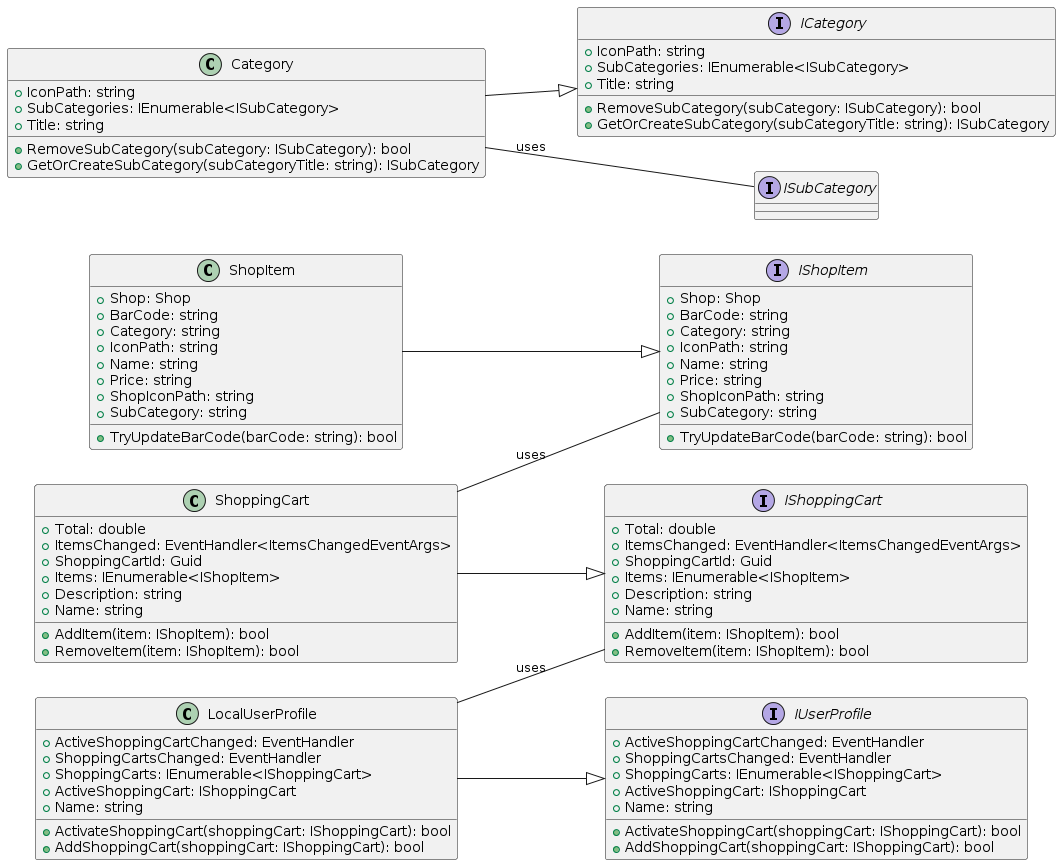
\includegraphics[width=1\linewidth]{img/app_models.png}
	\caption{Mobile App Models}
	\label{fig:appmodels}
\end{figure}

\subsubsection{Presentation Layer (View, ViewModel)}

Due to the fact that both the View and ViewModel layers are accountable for the configuration of the user interface, they are discussed together in this instance. 

The user interface of the application can be broken down into four primary sections: \begin{itemize}
	\item the shell, which provides a menu for navigating between categories;
	\item the main page, which is in charge of presenting the items for a particular category;
	\item the barcode page, which is in charge of scanning barcodes;
	\item  and the user profile page, which is responsible for accessing shopping carts.
\end{itemize} 
Additionally there's a popup for searching for items by their name.

Since the application is heavily dependent on the MVVM design pattern, the ViewModels implement INotifyPropertyChanged in order to update the View with information about changed properties. Additionally, the ViewModels implement the IHandle interface in order to handle messages that are published by the EventAggregator. The Views are being initialized and registered through the use of ResolverService, and I have avoided using the code-behind as much as possible because doing so is also a violation of the pattern.

There are additional ViewModels which are not matched by their own Views. The reason behind this is that the models used in this case are not enough by themselves and they need an extra layer of presentation logic to make sense for the user interface.

The general architecture of the layer can be seen on figure \ref{fig:appviewmodels} below.

\begin{figure}[H]
	\centering
	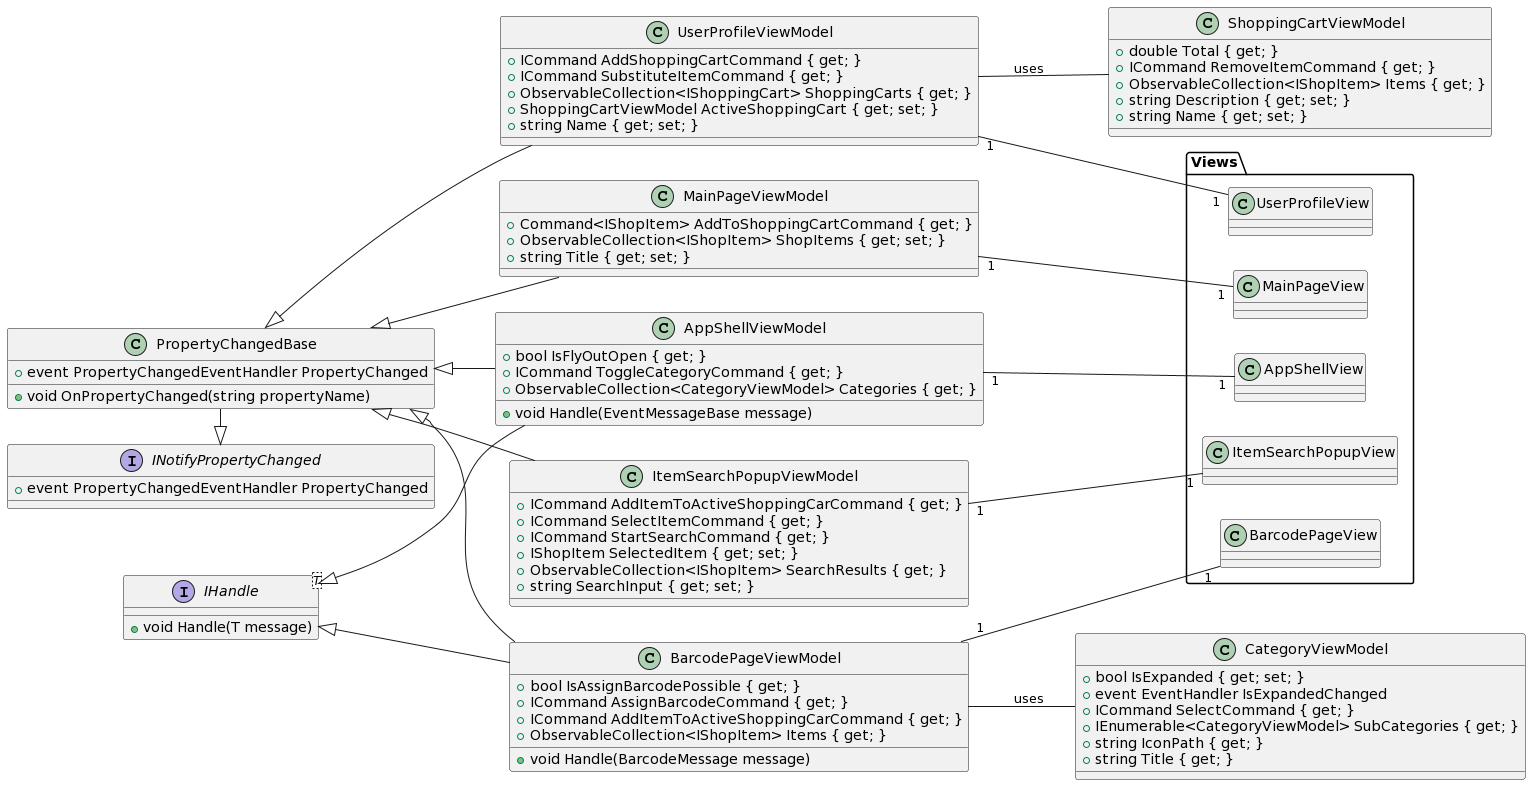
\includegraphics[width=1\linewidth]{img/app_viewmodels.png}
	\caption{Mobile App Views and ViewModels}
	\label{fig:appviewmodels}
\end{figure}

\noindent\textbf{Main page and Shell Fly-Out}

All of the items that fall under the chosen category are displayed on the main page. Every time a new category is chosen, the content is automatically updated in a dynamic manner. Each of these items displays the name of the store from which they originate and can be added to the shopping cart that is currently active. 

The flyout of the shell is utilized for the purpose of presenting the list of categories and subcategories that are available. The list of subcategories expands and shrinks depending on whether the main category is clicked on or not. 

The UI implementation is presented on figure \ref{fig:appitemspage} below.

\begin{figure}[H]
	\centering
	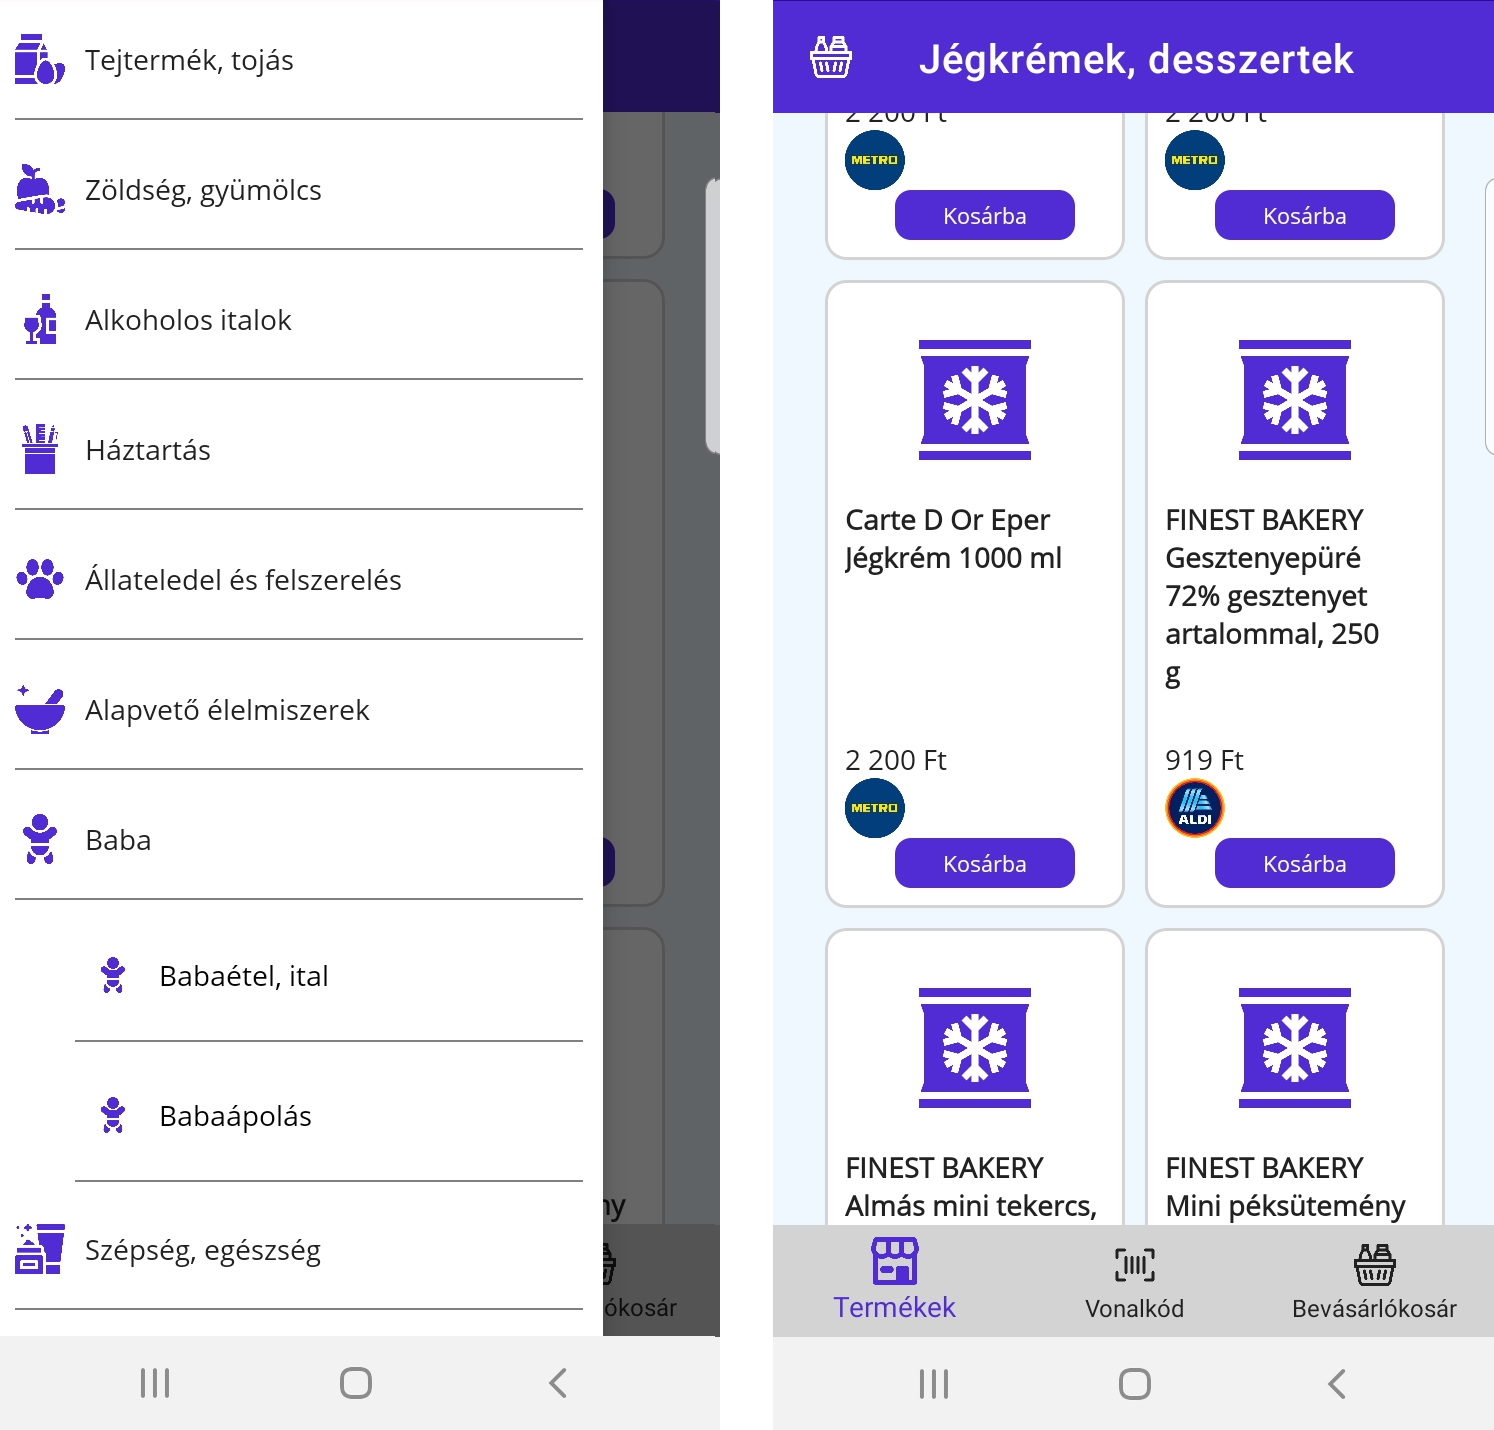
\includegraphics[width=0.5\linewidth]{img/app_itemspage.png}
	\caption{Mobile App Main Page and Shell Fly-out}
	\label{fig:appitemspage}
\end{figure}

\noindent\textbf{Barcode Page}

The barcode page includes a camera-view for reading item barcodes. After reading the code for an item, the app attempts to locate it in the repository. If it contains matching item(s), they are displayed and can be added to the current shopping cart. 

If no items match, the user can manually assign the code to any items that do not already have a code assigned. For this purpose, the search popup shown in figure \ref{fig:appsearchpopup} is used.

Figure \ref{fig:appbarcodepage} on the next page shows how the barcode page was implemented.

\begin{figure}[H]
	\centering
	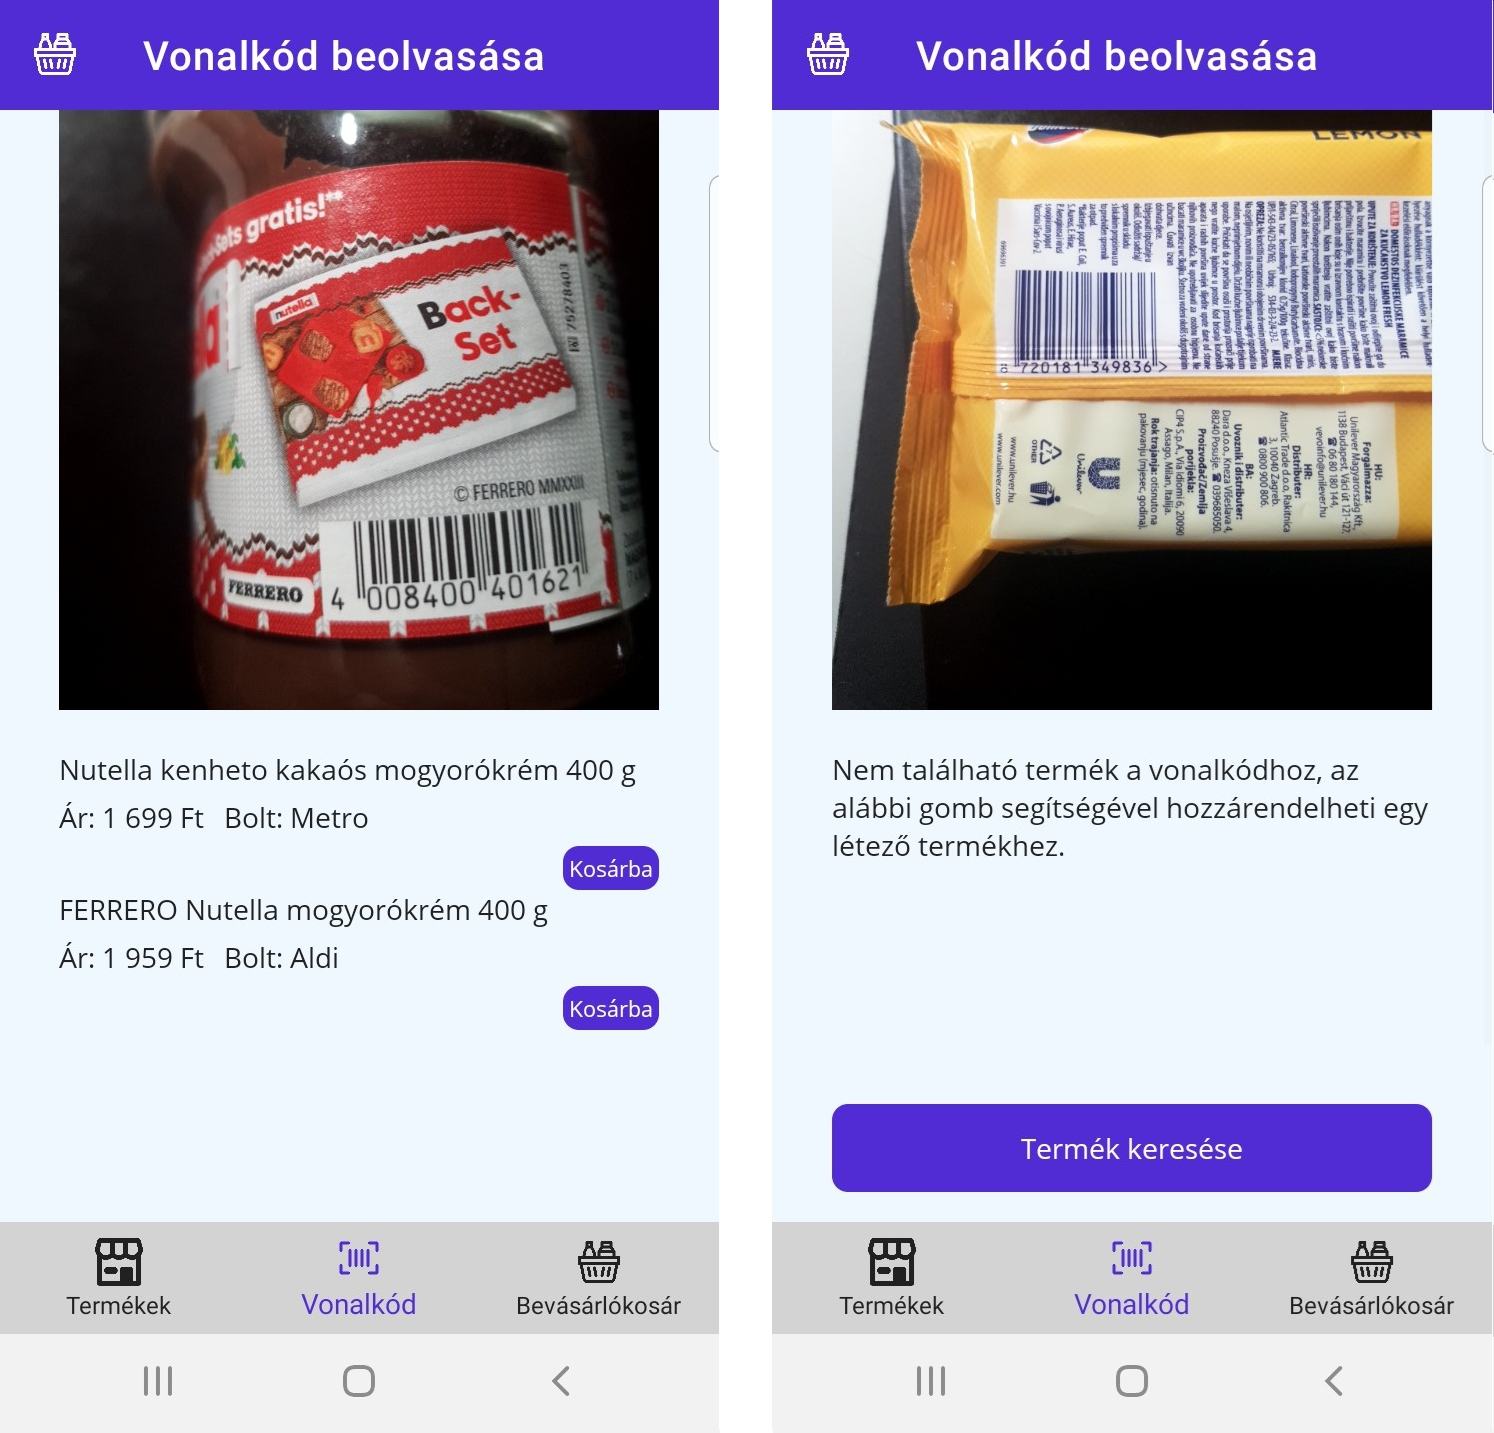
\includegraphics[width=0.6\linewidth]{img/app_barcodepage.png}
	\caption{Mobile App Barcode Page}
	\label{fig:appbarcodepage}
\end{figure}

\noindent\textbf{User profile / Shopping Carts Page}

\begin{figure}[H]
	\centering
	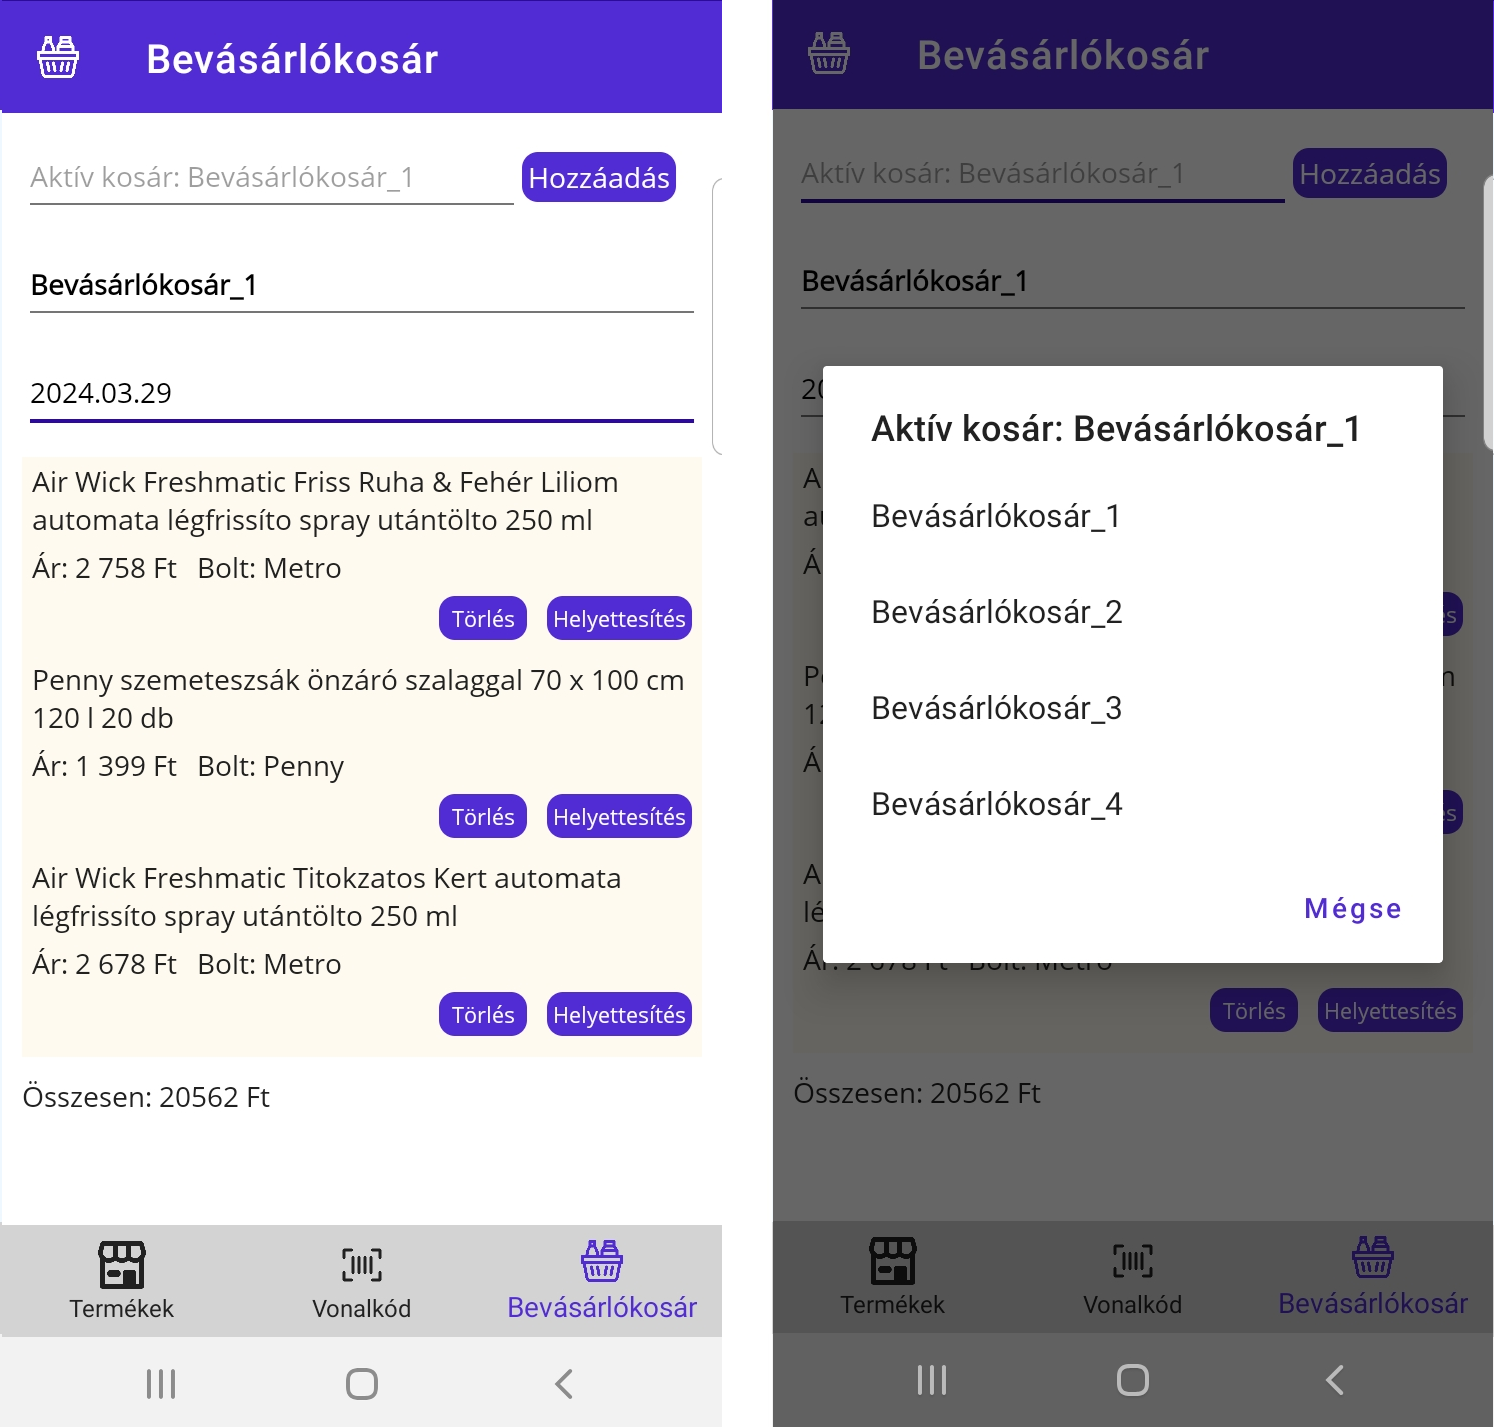
\includegraphics[width=0.6\linewidth]{img/app_shoppingcartpage.png}
	\caption{Mobile App User Profile Page}
	\label{fig:appshoppingcartspage}
\end{figure}

The way the presentation for the user profile and its associated shopping carts is implemented is visible on figure \ref{fig:appshoppingcartspage} above.

The page displays the active shopping cart and allows the user to switch between carts.  A scrollable popup allows users to switch between shopping carts. Selecting a shopping cart activates it. The shopping carts include metadata such as name and description. All shopping carts contain and store the items that the user adds to them. 

The shopping cart view shows the current items in the cart as well as the total number of items included; the user can also remove or substitute items. The substitution makes use of the previously mentioned item searching popup, as shown on figure \ref{fig:appsearchpopup}.

\noindent\textbf{Search Popup}

Finally, let's discuss the popup that allows the user to search for items stored in the repository. To return results, the search must contain at least three characters. If there are too many results, the user will be shown the top ten.  Scrolling through the popup reveals the hidden hits. 

The popup displays the select command for modules that use it. When an item is selected, the calling module receives the item's reference. It also includes a "Add to cart" command so that users can easily add items to their shopping cart if they discover something they forgot to add previously.

The realized user interface of the popup is visible on figure \ref{fig:appsearchpopup} below.

\begin{figure}[H]
	\centering
	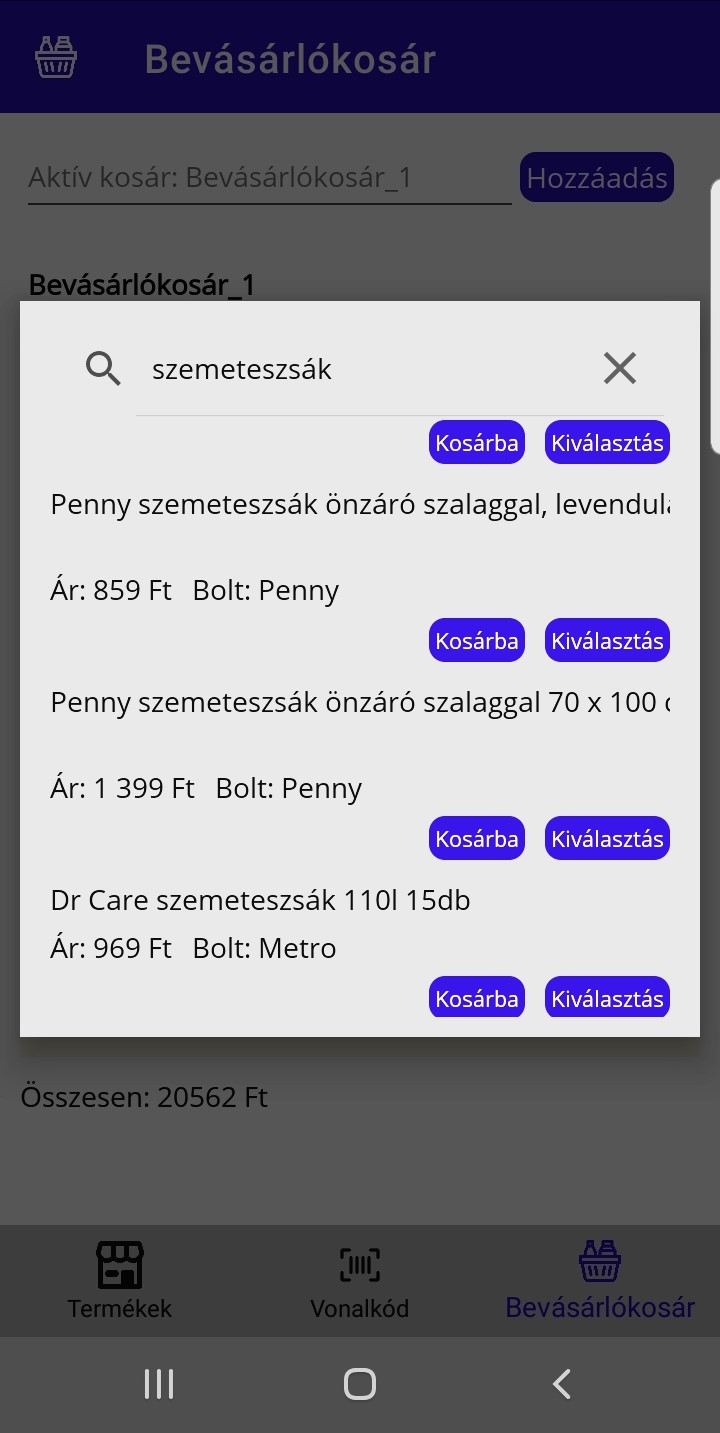
\includegraphics[width=0.3\linewidth]{img/app_search.png}
	\caption{Mobile App Search Popup}
	\label{fig:appsearchpopup}
\end{figure}